\documentclass[sigconf,review,anonymous]{acmart}

%% ---------------------------------------------------------------------------
%%  Architecture-as-Contract: A Substrate for Reviewable and Agentic
%%  Software Evolution in Monorepos.
%%  Initial draft targeting ACM FSE.
%% ---------------------------------------------------------------------------

\settopmatter{printacmref=false}
\setcopyright{none}
\renewcommand\footnotetextcopyrightpermission[1]{}
\pagestyle{plain}

%% ----- Packages ------------------------------------------------------------
\usepackage{tikz}
\usepackage{pgfplots}
\pgfplotsset{compat=1.18}
\usetikzlibrary{positioning,arrows.meta,calc,fit,backgrounds,shapes.geometric,decorations.pathreplacing,shadows.blur}
\usepackage{booktabs}
\let\Bbbk\relax
\usepackage{amsmath,amssymb}
\usepackage{mathtools}
\usepackage{microtype}
\usepackage{enumitem}

%% Define theorem environments explicitly (avoid relying on acmart option state).
\theoremstyle{plain}
\newtheorem{theorem}{Theorem}[section]
\newtheorem{lemma}[theorem]{Lemma}
\newtheorem{corollary}[theorem]{Corollary}
\newtheorem{property}[theorem]{Property}
\theoremstyle{definition}
\newtheorem{definition}[theorem]{Definition}
\newtheorem{assumption}{Assumption}

%% ----- A restrained, print-safe palette (Healy/Bostock sensibility) --------
%% Cool neutral ink, one warm accent for "danger/boundary", one cool accent
%% for "safe/interior". Backgrounds are desaturated washes, never saturated.
\definecolor{ink}{HTML}{1A1F24}        % near-black text/structure
\definecolor{slate}{HTML}{5B6B7A}      % secondary lines/labels
\definecolor{mist}{HTML}{E9EDF1}       % light fill for containers
\definecolor{mist2}{HTML}{D7DEE6}      % slightly darker container fill
\definecolor{steel}{HTML}{3D6A99}      % primary accent (safe / structural)
\definecolor{steelwash}{HTML}{E2EBF3}  % steel wash
\definecolor{rust}{HTML}{B5532A}       % warning accent (boundary / danger)
\definecolor{rustwash}{HTML}{F4E4DB}   % rust wash
\definecolor{moss}{HTML}{4E7A4E}       % "accepted / pass"
\definecolor{mosswash}{HTML}{E3EEE3}

%% ----- Shared TikZ styles --------------------------------------------------
%% Every figure draws from these so the paper has one visual language.
\tikzset{
  font=\sffamily,
  >=Stealth,
  %% nodes
  box/.style        = {rounded corners=2pt, draw=ink, line width=0.6pt,
                       fill=white, inner sep=5pt, align=center},
  container/.style  = {rounded corners=3pt, draw=slate, line width=0.6pt,
                       fill=mist, inner sep=8pt},
  leaf/.style       = {rounded corners=2pt, draw=steel, line width=0.6pt,
                       fill=steelwash, inner sep=4pt, align=center,
                       font=\sffamily\small},
  gate/.style       = {rounded corners=2pt, draw=ink, line width=0.7pt,
                       fill=white, inner sep=6pt, align=center},
  %% arrows
  dep/.style        = {->, draw=slate, line width=0.7pt},
  depnew/.style     = {->, draw=rust, line width=1.1pt},
  flow/.style       = {->, draw=ink, line width=0.8pt},
  agg/.style        = {-, draw=slate, line width=0.5pt, dotted},
  %% annotations
  lbl/.style        = {font=\sffamily\footnotesize, text=slate},
  caption/.style    = {font=\sffamily\small, text=ink},
}

\begin{document}

\title{Architecture as Contract: A Hierarchical Graph Substrate
for Reviewable and Agentic Software Evolution}

\author{Anonymous Author(s)}
\affiliation{%
  \institution{Submitted for review}
  \country{}
}

\renewcommand{\shortauthors}{Anon.}

\begin{abstract}
Large repositories evolve through a steady stream of local edits, cross-cutting
refactorings, and, increasingly, changes proposed by coding agents. Human
review remains the main mechanism for protecting architectural intent, but the
artifact reviewers usually have is a textual diff. That diff is often a poor
proxy for the question reviewers actually need to answer: did this change alter
a module boundary, introduce a dependency, or widen an interface that other
parts of the system may rely on? Architecture diagrams express those concerns,
but in most projects they are informal drawings rather than checked artifacts
connected to the code.

We present \textsc{Archon}, a substrate for treating architecture as a
versioned, mechanically checked contract. \textsc{Archon} represents a
repository as a \emph{hierarchical attributed graph}: boxes nest from packages
down to functions, dependency arrows aggregate along the containment tree, and
nodes carry structural contracts describing their public surface and permitted
dependencies. Where automated evolution is intended, nodes may also carry
behavioral contracts stated over that surface. The unit of review is a
\emph{graph delta} projected to the altitude at which the change should be
understood. We formalize the model, define node identity across refactorings,
and state a boundary-locality theorem: under explicit assumptions about
encapsulation and contract adequacy, an implementation change with an empty
boundary delta and a preserved behavioral contract is unobservable outside the
box. The theorem is not a claim that current repositories satisfy these
assumptions automatically; rather, it identifies the checks and evidence needed
to make autonomous internal evolution defensible. We separate this fixed
substrate from the open set of proposers, including humans, coding agents, and
search-based systems, and outline the empirical studies needed to evaluate the
approach across Go, Rust, and Python monorepos.
\end{abstract}

\begin{CCSXML}
<ccs2012>
<concept><concept_id>10011007.10011006.10011008</concept_id>
<concept_desc>Software and its engineering~Software architectures</concept_desc>
<concept_significance>500</concept_significance></concept>
<concept><concept_id>10011007.10010940.10010992</concept_id>
<concept_desc>Software and its engineering~Software verification</concept_desc>
<concept_significance>300</concept_significance></concept>
<concept><concept_id>10011007.10011074.10011099</concept_id>
<concept_desc>Software and its engineering~Software evolution</concept_desc>
<concept_significance>500</concept_significance></concept>
</ccs2012>
\end{CCSXML}
\ccsdesc[500]{Software and its engineering~Software architectures}
\ccsdesc[500]{Software and its engineering~Software evolution}
\ccsdesc[300]{Software and its engineering~Software verification}

\keywords{software architecture, monorepos, dependency analysis,
architectural conformance, automated program evolution, code review}

\maketitle

%% ===========================================================================
\section{Introduction}
%% ===========================================================================

Engineers reason about software with boxes and arrows. A box is a unit of the
system: a service, a package, a class. An arrow is a dependency between two
units. This vocabulary underlies architecture whiteboards, onboarding talks, and
formal notations from UML package diagrams to the C4 model~\cite{c4model}. Yet
in many projects the picture remains a \emph{drawing}. It records intent, but it
is not mechanically connected to the code, and it can diverge from the system it
describes. The authoritative description of the architecture, namely what
actually imports, calls, or exposes what, is scattered through the source. It is
legible to compilers and language servers, but not in the form that a reviewer
or an automated proposer needs when evaluating architectural risk.

This gap matters more in large repositories. Monorepos make cross-cutting change
practical by placing many components in one versioned
space~\cite{potvin2016google,jaspan2018advantages}. The same affordance also
makes architectural erosion easy: a new import can cross a boundary that was
understood socially but never represented as an enforceable rule. Coding agents
add a second pressure. They can produce changes at the granularity of functions
or methods, often in large textual diffs whose architectural effect is small,
ambiguous, or accidentally broad. For both human and machine-authored changes,
the important review question is not simply how many lines changed. It is
whether the change alters a boundary that other parts of the system depend on.

\paragraph{Thesis.}
We argue that the boxes-and-arrows view should become a \emph{first-class,
versioned, mechanically checked artifact} serving three related uses:
\begin{enumerate}[leftmargin=1.4em,itemsep=2pt,topsep=2pt]
\item \textbf{documentation}: a zoomable picture of the system derived from the
source rather than maintained separately;
\item \textbf{review}: a per-change \emph{architectural delta} that tells a
reviewer which boxes, arrows, and surfaces a pull request changes at the
altitude where that change is legible; and
\item \textbf{evolution}: the contract against which automated proposers are
checked before their changes are admitted.
\end{enumerate}
The useful observation is that these need not be three different systems. If the
same artifact documents the repository, defines the review delta, and supplies
the boundary checked for automated changes, then humans and tools share the same
architectural vocabulary.

\paragraph{Approach.}
We represent a repository as a \emph{hierarchical attributed graph}
(\S\ref{sec:model}). Boxes nest along a containment tree---repository
$\supseteq$ package $\supseteq$ module $\supseteq$ function---and arrows exist at
every level, with a coarse arrow defined as the \emph{aggregation} of the finer
arrows beneath it (Figure~\ref{fig:aggregation}). This single structure
reconciles the two granularities that the problem demands: humans review at the
package altitude, agents evolve at the function altitude, and the two are
\emph{projections of the same graph} rather than separate models that can drift
apart. Each node carries a \emph{structural contract}---its public surface and
the dependencies it is permitted to have---and, where we intend to automate its
evolution, a \emph{behavioral contract}: properties stated \emph{purely over its
public surface}. A change is gated by its \emph{graph delta}, computed by
extracting the graph before and after and diffing the two; gating decisions are
made per-altitude, so a change that is a thousand-line internal rewrite at the
function level can be \emph{empty} at the package level and reviewed as such.

\paragraph{The safety argument.}
The model also makes explicit what must be true before internal automation can
be treated as low risk. We define node identity to be stable under the moves and
renames that refactoring and agents perform (\S\ref{sec:identity}); otherwise a
routine refactor would appear as deletion plus creation and architectural deltas
would be noisy. We then state and prove \emph{boundary locality}
(\S\ref{sec:guarantees}): if a change leaves a box's boundary delta empty and
preserves the box's behavioral contract, then, under explicit assumptions about
encapsulation and contract adequacy, the change is unobservable to other boxes.
This is a familiar modularity intuition, but the graph substrate turns it into a
checkable review condition: first establish that the boundary did not move, then
check the behavioral obligations that justify treating the implementation as
substitutable.

\paragraph{Separating the fixed from the open.}
A substrate for automated evolution should not depend on a particular agent or
search procedure. We therefore separate five concerns
(Figure~\ref{fig:substrate}) into a \emph{fixed substrate}: extraction,
representation, structural conformance, and behavioral verification, and an
\emph{open} space of \emph{proposers}: humans, coding agents, and synthesis or
search systems such as those targeted by \textsc{nous} and \textsc{skydiscover}.
Every proposer emits the same kind of artifact, a graph delta plus a code
change, and is evaluated by the same gates. The point is not to predict which
proposer will be best, but to make the acceptance boundary independent of the
proposer.

\paragraph{Contributions.}
\begin{itemize}[leftmargin=1.4em,itemsep=3pt,topsep=2pt]
\item A \emph{hierarchical attributed graph} model of a repository that unifies
documentation, review, and agentic evolution as consumers of one versioned
artifact, with arrows and contracts that aggregate along a containment tree
(\S\ref{sec:model}).
\item A definition of \emph{node identity} stable under rename and move, which
makes architectural deltas signal rather than noise and makes ``the boundary
did not change'' computable (\S\ref{sec:identity}).
\item A \emph{boundary-locality theorem} with proof sketch and explicit
assumptions: an empty boundary delta plus a preserved behavioral contract
implies unobservability to the rest of the system under those assumptions,
providing the conditional basis for fine-grained autonomous evolution under
coarse-grained human review
(\S\ref{sec:guarantees}).
\item A \emph{conformance regime} of composable gates: an acyclicity policy, a
per-altitude spread gate that bounds review blast radius, and a surface gate,
together with an evolution protocol that routes
boundary-preserving changes to automated gates and boundary-changing changes to
human review of the delta (\S\ref{sec:enforce},~\S\ref{sec:evolve}).
\item A concrete \emph{evaluation plan} across Go, Rust, and Python monorepos,
including retrospective pull-request studies, implementation case studies, and
agentic evolution experiments focused on behavioral-contract coverage
(\S\ref{sec:eval},~\S\ref{sec:agenda}).
\end{itemize}

We name the substrate \textsc{Archon}. This paper presents the model, the
conditional guarantee it supports, and the empirical plan needed to test whether
the required assumptions are practical in real repositories.

%% ===========================================================================
\section{Overview and Running Example}\label{sec:overview}
%% ===========================================================================

We draw our running example from \textsc{vLLM}~\cite{kwon2023vllm}, a
high-throughput LLM inference engine and a representative modern monorepo. Its
execution layer, the package \texttt{executor}, depends on its scheduling layer,
\texttt{core/sched}. Concretely, \texttt{Executor.execute\_model()} takes a
\texttt{SchedulerOutput} and \texttt{Executor.sample\_tokens()} takes a
\texttt{GrammarOutput}, both types defined in \texttt{core/sched}. At the
granularity an agent works in, these are distinct, type-driven import edges
among leaf entities (functions and classes). At the granularity a human reviews
in, they are a \emph{single} fact: \texttt{executor} depends on
\texttt{core/sched}. Figure~\ref{fig:aggregation} shows both views and the
relation between them. The package-level arrow is not a separate, hand-drawn
claim that might disagree with the code; it is the \emph{aggregation} of the
leaf-level edges, recomputed from the source on every change. This is the
property that keeps the documentation honest and the review legible at once.

Now suppose an evolution agent rewrites \texttt{execute\_model} to batch its
forward passes for throughput. At the leaf altitude this may be a large
implementation diff. At the package altitude it may be \emph{empty}: the set of
edges from \texttt{executor} to \texttt{core/sched} is unchanged, and the
function's signature is unchanged. We want a system in which
(i)~the reviewer can see that the cross-package architecture did not change, and
(ii)~the automated gate can distinguish this case from a rewrite that quietly
adds a dependency or widens an interface. If the relevant behavioral obligations
also hold, the system has a principled basis for treating the change as internal.
Sections~\ref{sec:model}--\ref{sec:guarantees} build this model; the present
section fixes intuitions and notation.

Throughout, we distinguish the \emph{actual} graph, extracted mechanically from
source and thus always faithful to the code, from the \emph{intended} graph, a
declared baseline that the actual graph is checked against. A pull request is
\emph{conformant} when the actual graph stays within what the intended graph
permits. For a greenfield repository, the intended graph may be written before
or alongside the first implementation. For a brownfield repository, which is the
more common and more difficult case, the intended graph is seeded by snapshotting
the actual graph (\S\ref{sec:enforce}); it then advances only through reviewed
deltas, so it encodes accumulated architectural intent without anyone having to
draw the whole architecture up front. This makes adoption descriptive before it
is prescriptive: first make the existing architecture visible, then decide which
future deltas are allowed.

%% ===========================================================================
\section{The Hierarchical Attributed Graph}\label{sec:model}
%% ===========================================================================

We model a repository state as a single artifact that carries structure
(boxes and arrows), hierarchy (boxes nest), and contracts (what each box
promises). We build it up in layers.

\subsection{Boxes, the containment tree, and arrows}

\begin{definition}[Architecture graph]\label{def:graph}
An \emph{architecture graph} is a tuple
$G = (V,\;\mathsf{par},\;E,\;\sigma)$ where
\begin{itemize}[leftmargin=1.4em,itemsep=1pt,topsep=2pt]
\item $V$ is a finite set of \emph{nodes} (boxes), each a unit of the system
at some altitude---repository, package, module/file, or leaf
(function, method, type, interface);
\item $\mathsf{par}:V \rightharpoonup V$ is a partial \emph{parent} map whose
graph is a rooted tree $T$ (the \emph{containment tree}): $\mathsf{par}(v)$ is
the box that directly contains $v$, undefined only at the root $r$;
\item $E \subseteq V \times V$ is a set of directed \emph{arrows}
(dependencies); and
\item $\sigma$ assigns to each node its \emph{attributes}, including its
public surface and contracts (\S\ref{sec:contracts}).
\end{itemize}
We write $u \sqsubseteq v$ when $u$ is $v$ or a descendant of $v$ in $T$, and
$\mathsf{leaves}(v)=\{\ell : \ell \sqsubseteq v,\ \ell \text{ a leaf}\}$.
\end{definition}

The containment tree is what gives the model its two-altitude character: a
human reads a \emph{cut} of $T$ near the root (packages), an agent operates on
the leaves, and both are views of the same $V$.

\paragraph{Edges live at the leaves; coarse arrows are derived.}
We take the \emph{primitive} dependencies to be those the compiler or
type-checker actually sees---one leaf referring to another (a call, a field
access, an implemented interface). Formally $E$ is given at the leaf level, and
arrows between interior boxes are defined by \emph{aggregation}.

\begin{definition}[Arrow aggregation / projection]\label{def:agg}
For boxes $a,b \in V$ with $a \neq b$ and neither containing the other, the
\emph{aggregated arrow} $a \Rightarrow b$ exists iff some leaf of $a$ depends on
some leaf of $b$:
\[
a \Rightarrow b \quad\Longleftrightarrow\quad
\exists\, \ell_a \in \mathsf{leaves}(a),\ \ell_b \in \mathsf{leaves}(b)
\;:\; (\ell_a,\ell_b)\in E .
\]
The \emph{witness set} $W(a\!\Rightarrow\! b)=\{(\ell_a,\ell_b)\in E :
\ell_a\sqsubseteq a,\ \ell_b\sqsubseteq b\}$ records the leaf edges the arrow
summarizes. The \emph{projection} of $G$ to an antichain $A\subseteq V$ of $T$
(a set of boxes, no one containing another, covering all leaves) is the graph
on $A$ whose arrows are the aggregated arrows among members of $A$.
\end{definition}

Projection is the formal meaning of ``zoom'': choosing the antichain of all
packages yields the human's review diagram; choosing the antichain of all
leaves yields the agent's working graph. Because every coarse arrow carries its
witness set, the human can expand any arrow to see exactly which leaf
dependencies realize it (Figure~\ref{fig:aggregation}), and---crucially---a
change that does not alter $E$ within $W(a\!\Rightarrow\! b)$ cannot alter the
arrow $a\!\Rightarrow\! b$.

\subsection{Public surface and well-formedness}

A box hides its interior and exposes a surface. We make the surface explicit
because it, not the box's code, is what other boxes may depend on.

\begin{definition}[Public surface]\label{def:surface}
The \emph{public surface} $\mathsf{surf}(v)$ of a box $v$ is the set of its
entities (and their types/signatures) that are visible outside $v$. We require
graphs to be \emph{encapsulated}: every cross-box leaf edge enters its target
box through that box's surface. Formally, if $(\ell_a,\ell_b)\in E$ and the
nearest common ancestor of $\ell_a,\ell_b$ is a proper ancestor of $\ell_b$'s
parent box $b'$, then $\ell_b \in \mathsf{surf}(b')$.
\end{definition}

Encapsulation is what language mechanisms such as Go internal packages, Rust's
\texttt{pub(crate)} visibility, and Python's \texttt{\_\_all\_\_} conventions
approximate; an extractor can read these signals to compute
$\mathsf{surf}$. A graph is \emph{well-formed} if it is encapsulated and its
\emph{package-level projection satisfies the repository's cycle policy};
\S\ref{sec:enforce} discusses the strict acyclic policy used in the base model
and the empirical need to study migration paths for existing cyclic graphs.

%% ---- Figure 1: aggregation (real) ----------------------------------------
\begin{figure}[t]
\centering
%% Figure: arrow aggregation across two altitudes -- real vLLM example.
%% Column-width layout (fits ~241pt). executor depends on core/sched.
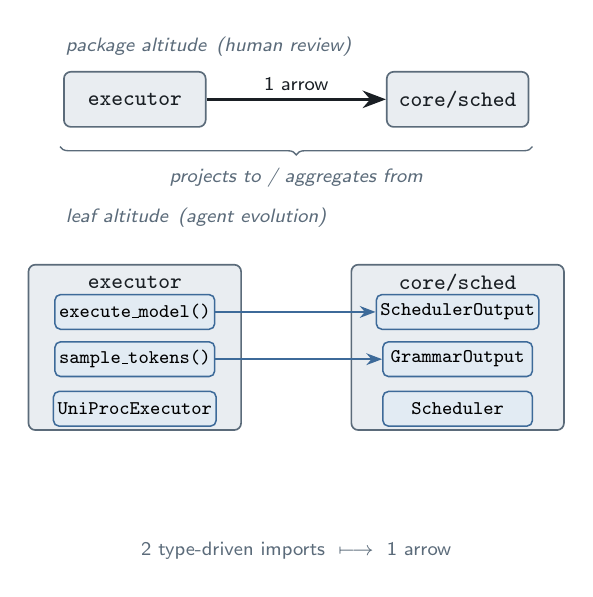
\begin{tikzpicture}[
  pkg/.style    = {rounded corners=2.5pt, draw=slate, line width=0.6pt, fill=mist, inner sep=4pt},
  leafn/.style  = {rounded corners=2pt, draw=steel, line width=0.55pt, fill=steelwash,
                   inner sep=1.5pt, align=center, font=\sffamily\fontsize{6.6}{7.6}\selectfont\ttfamily,
                   minimum width=19mm, minimum height=4.4mm},
  depagg/.style = {->, draw=ink, line width=1.2pt},
  fine/.style   = {->, draw=steel, line width=0.6pt},
  lbl/.style    = {font=\sffamily\scriptsize, text=slate},
  lblb/.style   = {font=\sffamily\footnotesize, text=ink},
]

%% ============ coarse (human) altitude ============
\node[lbl, anchor=west] at (-0.05,1.62) {\itshape package altitude \textcolor{slate}{\,(human review)}};
\node[pkg, minimum width=18mm, minimum height=7mm] (Pexec) at (0.95,0.95) {};
\node[lblb] at (Pexec.center) {\textbf{\texttt{executor}}};
\node[pkg, minimum width=18mm, minimum height=7mm] (Pcore) at (5.05,0.95) {};
\node[lblb] at (Pcore.center) {\textbf{\texttt{core/sched}}};
\draw[depagg] (Pexec.east) -- node[lbl, above, text=ink, yshift=-0.3mm] {1 arrow} (Pcore.west);

%% ============ projection brace ============
\draw[decorate, decoration={brace, amplitude=3pt, mirror}, slate, line width=0.5pt]
   (0.0,0.35) -- (6.0,0.35);
\node[lbl] at (3.0,-0.05) {\itshape projects to / aggregates from};

%% ============ fine (agent) altitude ============
\node[lbl, anchor=west] at (-0.05,-0.55) {\itshape leaf altitude \textcolor{slate}{\,(agent evolution)}};
\begin{scope}[yshift=-0.2cm]
  \node[pkg, minimum width=27mm, minimum height=21mm] (Ecl) at (0.95,-2.0) {};
  \node[lblb] at (Ecl.north) [yshift=-2.4mm] {\textbf{\texttt{executor}}};
  \node[leafn] (exec)   at (0.95,-1.55) {execute\_model()};
  \node[leafn] (sample) at (0.95,-2.15) {sample\_tokens()};
  \node[leafn] (uniproc)at (0.95,-2.78) {UniProcExecutor};

  \node[pkg, minimum width=27mm, minimum height=21mm] (Ccl) at (5.05,-2.0) {};
  \node[lblb] at (Ccl.north) [yshift=-2.4mm] {\textbf{\texttt{core/sched}}};
  \node[leafn] (sout)   at (5.05,-1.55) {SchedulerOutput};
  \node[leafn] (gout)   at (5.05,-2.15) {GrammarOutput};
  \node[leafn] (sched)  at (5.05,-2.78) {Scheduler};

  %% two parallel, non-crossing edges
  \draw[fine] (exec.east)   -- (sout.west);
  \draw[fine] (sample.east) -- (gout.west);
\end{scope}
\node[lbl] at (3.0,-4.78) {2 type-driven imports $\;\longmapsto\;$ 1 arrow};

\end{tikzpicture}

\caption{One graph, two altitudes, drawn from \textsc{vLLM}. Two type-driven
leaf-level import edges (bottom, where agents work)---\texttt{execute\_model()}
consuming \texttt{SchedulerOutput} and \texttt{sample\_tokens()} consuming
\texttt{GrammarOutput}---aggregate to a single package-level arrow
\texttt{executor}\,$\Rightarrow$\,\texttt{core/sched} (top, where humans review).
The arrow carries the witness set of leaf edges it summarizes, so a change that
does not touch those edges cannot change the arrow.}
\label{fig:aggregation}
\end{figure}

\subsection{Contracts: structural and behavioral}\label{sec:contracts}

Attributes $\sigma(v)$ carry two contracts per box, and optionally one per
arrow.

\begin{definition}[Structural contract]
The \emph{structural contract} of a box $v$ is the pair
$\mathsf{SC}(v)=\big(\mathsf{surf}(v),\,\mathsf{Allow}(v)\big)$, where
$\mathsf{surf}(v)$ is its public surface and $\mathsf{Allow}(v)\subseteq V$ is
the set of boxes $v$ is permitted to depend on (its allowed out-arrows). A box
\emph{satisfies} its structural contract when its actual surface is a subset of
the declared one and its actual out-arrows target only allowed boxes.
\end{definition}

\begin{definition}[Behavioral contract]\label{def:bc}
A \emph{behavioral contract} $\mathsf{BC}(v)$ of a box $v$ is a set of
properties over the observable behavior of $v$ \emph{at its public surface}:
predicates relating the inputs and outputs (and externally visible effects) of
the entities in $\mathsf{surf}(v)$. A behavioral contract may not refer to any
entity not in $\mathsf{surf}(v)$.
\end{definition}

The surface-only restriction in Definition~\ref{def:bc} is deliberate and
load-bearing: a property that mentions a box's internals is not a contract but
a test of a particular implementation, and it would forbid exactly the internal
evolution we want to enable. Contracts at the surface are the obligations a
box's neighbors are entitled to rely on; everything else is free to change. We
return to this in \S\ref{sec:guarantees}, where it underwrites the safety
theorem. An \emph{arrow contract} on $a\!\Rightarrow\! b$ is a consumer-driven
contract~\cite{fowler2006cdc}: the subset of $\mathsf{BC}(b)$ that $a$ actually
relies upon, which lets $b$ evolve freely so long as that subset holds.

\paragraph{Aggregating contracts up the tree.}
Arrows aggregate mechanically (Definition~\ref{def:agg}); contracts do not. We
\emph{state} a parent's behavioral contract independently at its own surface
rather than deriving it as the conjunction of its children's. Deriving it would
re-expose child internals at the parent boundary and forbid reorganizing
children---the opposite of what hierarchy is for. Thus $\mathsf{BC}(\textsf{package})$
constrains only the package's public surface, and the package's children may be
refactored arbitrarily as long as that surface contract continues to hold. This
asymmetry (arrows aggregate, contracts are restated) is a design decision we
revisit in \S\ref{sec:agenda}.

%% ===========================================================================
\section{Node Identity Under Refactoring}\label{sec:identity}
%% ===========================================================================

Everything downstream---legible diffs, the ``boundary unchanged'' check, the
safety theorem---rests on being able to say that a node \emph{after} a change
is ``the same node'' as one before, even though refactoring and agents
routinely rename entities and move them between files. If identity were keyed on
qualified path, then moving \texttt{execute\_model} from one executor file to
another would read as deleting one function and creating another: a maximal,
alarming delta for a no-op refactor, and worse, a spurious change to every
arrow incident on it. The delta would be noise, and ``the boundary did not
change'' would be uncomputable. We therefore make identity a first-class,
inferred relation rather than a syntactic key.

\begin{definition}[Identity correspondence]\label{def:identity}
Let $G,G'$ be the graphs before and after a change. An \emph{identity
correspondence} is a partial injection $\iota : V \rightharpoonup V'$ matching
nodes that denote the same architectural entity across the change. Nodes
outside $\mathrm{dom}(\iota)$ are \emph{deleted}; nodes outside
$\mathrm{range}(\iota)$ are \emph{created}; a matched pair $(v,\iota(v))$ is
\emph{renamed} if their names differ, \emph{moved} if their parents differ
(i.e.\ $\iota(\mathsf{par}(v)) \neq \mathsf{par}'(\iota(v))$), and
\emph{internally changed} if the leaf's body differs.
\end{definition}

We infer $\iota$ rather than trusting names, combining three signals in
decreasing order of authority:

\begin{enumerate}[leftmargin=1.4em,itemsep=2pt,topsep=2pt]
\item \textbf{Stable identifiers when available.} Some toolchains expose
durable symbol identifiers (e.g.\ a mangled symbol or a USR-style key) that
survive moves; when present they pin $\iota$ directly.
\item \textbf{Surface and signature match.} A leaf whose signature (name aside)
and incident edges are preserved is strong evidence of correspondence, even
across a rename.
\item \textbf{Tree-edit similarity.} For the residual, we match on structural
similarity of the entity's syntax tree using a fine-grained tree-differencing
algorithm in the style of \textsc{GumTree}~\cite{falleri2014finegrained},
thresholded to avoid coincidental matches.
\end{enumerate}

The contract that matters for the rest of the paper is the property $\iota$
must satisfy, not the particular heuristic used to compute it:

\begin{property}[Identity stability]\label{prop:identity}
A pure rename or move---a change that alters only $\mathsf{par}$ or the name of
a node, leaving its public signature, its body, and the set of edges incident
on it unchanged up to $\iota$---induces \emph{no} created or deleted nodes and
\emph{no} change to any aggregated arrow.
\end{property}

\noindent
Property~\ref{prop:identity} is what makes a refactor diff as a refactor.
\S\ref{sec:eval} treats the empirical accuracy of $\iota$ (its precision and
recall against developer-labeled refactorings) as a first-class research
question, since the value of every delta the system reports is bounded by it.
We are explicit about the failure mode: an \emph{incorrect} $\iota$ does not
threaten \emph{safety}---the structural and behavioral gates still run on the
post-change graph regardless of how nodes were matched---but it degrades
\emph{legibility}, surfacing a clean refactor as a noisy delta. Safety depends
on the gates; identity governs only how clearly the change is presented and
whether it qualifies for the boundary-preserving fast path of
\S\ref{sec:evolve}.

%% ===========================================================================
\section{Separation of Concerns}\label{sec:concerns}
%% ===========================================================================

The model of \S\ref{sec:model}--\ref{sec:identity} is realized by five
concerns (Figure~\ref{fig:substrate}). Four are a \emph{fixed substrate}; the
fifth is deliberately \emph{open}.

\begin{description}[leftmargin=0em,itemsep=2pt,topsep=2pt,style=nextline]
\item[\textsf{1.\ Extraction} (language $\to$ graph)] Parses source into the
\emph{actual} graph---nodes at all altitudes, leaf edges, surfaces. This is the
\emph{only} language-specific concern; its output is language-neutral. It
reports facts and decides no policy.
\item[\textsf{2.\ Representation} (the artifact)] The versioned hierarchical
graph: the single object all other concerns read. It stores structure and
contracts, not source, and must diff, address any node stably
(\S\ref{sec:identity}), and project to any altitude (Definition~\ref{def:agg}).
\item[\textsf{3.\ Conformance} (structural gate)] Given two graph versions and
the declared rules, emits pass/fail: acyclicity, per-altitude spread, surface
(\S\ref{sec:enforce}). Purely structural---fast, total, deterministic.
\item[\textsf{4.\ Verification} (behavioral gate)] Holds a box's behavioral
contract while its internals change (\S\ref{sec:guarantees}). Grows lazily,
per box, as automation ambition grows.
\item[\textsf{5.\ Evolution} (proposers)] Anything that proposes a change: a
human, a coding agent, a synthesis or search system. \emph{Open by design.}
\end{description}

The discipline that makes the substrate reusable is stated as an invariant on
concern~5:

\begin{property}[Single funnel]\label{prop:funnel}
Every proposer's output is a pair (graph delta, code change), and a proposal is
accepted if and only if it passes the gates of concerns~3 and~4. No proposer
has any other path to acceptance.
\end{property}

\noindent
Property~\ref{prop:funnel} is what lets the substrate host evolutionary methods
that do not yet exist: a new agent framework can be placed in concern~5 without
changing concerns~1--4. Its proposals still encounter the same gates as
everyone else's. The gates are the contract between the repository and whatever
proposes changes to it.

%% ---- Figure 2: substrate (real) ----
\begin{figure}[t]
\centering
%% Figure: the five concerns -- fixed substrate vs. open proposers. Input by main.tex.
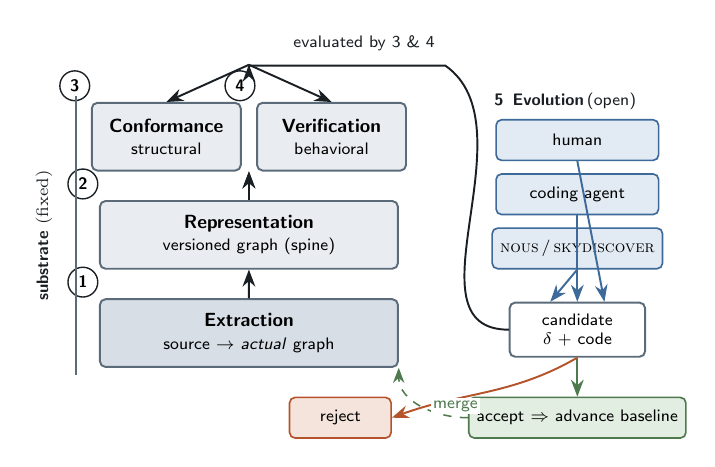
\begin{tikzpicture}[
  layer/.style = {rounded corners=2pt, draw=slate, line width=0.7pt,
                  minimum width=44mm, minimum height=10mm, align=center, fill=mist, font=\sffamily\footnotesize},
  num/.style   = {circle, draw=ink, line width=0.5pt, fill=white,
                  inner sep=0pt, minimum size=4.4mm, font=\sffamily\scriptsize\bfseries},
  prop/.style  = {rounded corners=2pt, draw=steel, line width=0.6pt, fill=steelwash,
                  minimum width=24mm, minimum height=6mm, align=center, font=\sffamily\scriptsize},
  gate/.style  = {rounded corners=2pt, draw=slate, line width=0.7pt, fill=white,
                  minimum width=20mm, minimum height=8mm, align=center, font=\sffamily\scriptsize},
  flow/.style  = {->, draw=ink, line width=0.7pt},
  lbl/.style   = {font=\sffamily\scriptsize, text=slate, align=left},
  scale=0.86, transform shape,
]

%% ---- substrate stack (left) ----
\node[layer, fill=mist2] (extract) at (0,0)
   {\textbf{Extraction}\\[0pt]{\scriptsize source $\to$ \emph{actual} graph}};
\node[layer] (repr) at (0,1.45)
   {\textbf{Representation}\\[0pt]{\scriptsize versioned graph (spine)}};
\node[layer, minimum width=22mm] (conf) at (-1.22,2.9)
   {\textbf{Conformance}\\[0pt]{\scriptsize structural}};
\node[layer, minimum width=22mm] (verif) at (1.22,2.9)
   {\textbf{Verification}\\[0pt]{\scriptsize behavioral}};

%% badges sit fully OUTSIDE the top-left corner so they never touch a title
\node[num] at ([xshift=-2.4mm,yshift=2.4mm]extract.north west) {1};
\node[num] at ([xshift=-2.4mm,yshift=2.4mm]repr.north west)    {2};
\node[num] at ([xshift=-2.4mm,yshift=2.4mm]conf.north west)    {3};
\node[num] at ([xshift=-2.4mm,yshift=2.4mm]verif.north west)   {4};

\draw[flow] (extract) -- (repr);
\draw[flow] (repr.north) -- (repr.north |- conf.south);
\draw[flow] (repr.north) -- (repr.north |- verif.south);

\draw[slate, line width=0.6pt] (-2.55,-0.62) -- (-2.55,3.5);
\node[lbl, rotate=90, anchor=south, text=ink] at (-2.78,1.44)
  {\itshape\bfseries substrate \normalfont(fixed)};

%% ---- proposers (right) ----
\node[lbl, text=ink, anchor=west] at (3.5,3.42) {\textbf{5\, Evolution}\,(open)};
\node[prop] (human)  at (4.85, 2.85) {human};
\node[prop] (agentA) at (4.85, 2.05) {coding agent};
\node[prop] (agentB) at (4.85, 1.25) {\textsc{nous}\,/\,\textsc{skydiscover}};

\node[gate, minimum width=20mm, minimum height=8mm] (cand) at (4.85,0.05)
   {candidate\\ $\delta$ + code};
\draw[flow, draw=steel] (human.south)  -- ([xshift=4mm]cand.north);
\draw[flow, draw=steel] (agentA.south) -- (cand.north);
\draw[flow, draw=steel] (agentB.south) -- ([xshift=-4mm]cand.north);

%% candidate -> gates 3 & 4: leave from the candidate's LEFT, run along a
%% clear corridor above the stack, then fork down into both gates. The corridor
%% (y=3.95) sits above every box and label, so the path clobbers nothing.
\coordinate (gap) at ($(conf.north east)!0.5!(verif.north west) + (0,0.55)$);
\draw[flow] (cand.west) to[out=180,in=-35] (2.9,3.95) -| (gap);
\draw[->, draw=ink, line width=0.7pt] (gap) -- (conf.north);
\draw[->, draw=ink, line width=0.7pt] (gap) -- (verif.north);
\node[lbl, text=ink, anchor=south] at (1.7,4.05) {evaluated by 3 \& 4};

%% verdicts
\node[prop, fill=mosswash, draw=moss, minimum width=24mm] (acc) at (4.85,-1.25)
   {accept $\Rightarrow$ advance baseline};
\node[prop, fill=rustwash, draw=rust, minimum width=15mm] (rej) at (1.35,-1.25) {reject};
\draw[flow, draw=moss] (cand.south) -- (acc.north);
\draw[flow, draw=rust] (cand.south) to[out=-150,in=20] (rej.east);
\draw[->, draw=moss, line width=0.55pt, dashed] (acc.west) to[out=180,in=-90] (extract.south east);
\node[lbl, text=moss, anchor=south, fill=white, inner sep=1pt] at (3.05,-1.2) {merge};
\end{tikzpicture}

\caption{Five concerns. Concerns 1--4 form a \emph{fixed} substrate;
concern~5---the proposers---is \emph{open}. Every proposer, human or machine,
emits the same artifact (a graph delta plus code) and is admitted only through
the same structural and behavioral gates (Property~\ref{prop:funnel}).}
\label{fig:substrate}
\end{figure}

%% ===========================================================================
\section{The Graph Delta and Structural Conformance}\label{sec:enforce}
%% ===========================================================================

A pull request transforms the actual graph from $G$ to $G'$. The unit of
review and gating is not the textual diff but the \emph{graph delta}.

\begin{definition}[Graph delta]\label{def:delta}
Given $G,G'$ and identity correspondence $\iota$ (\S\ref{sec:identity}), the
\emph{delta} $\Delta(G,G')$ is the labeled set of changes:
nodes created/deleted, nodes renamed/moved/internally-changed, arrows
added/removed/reversed, and surfaces widened/narrowed---each computed up to
$\iota$. The \emph{delta at altitude $A$} (an antichain of $T$) is the delta of
the projections, $\Delta(\pi_A G,\ \pi_A G')$.
\end{definition}

The same physical change has different deltas at different altitudes
(\S\ref{sec:overview}): a leaf-body rewrite has a nonempty delta at the leaf
altitude and an \emph{empty} delta at the package altitude. This is precisely
what lets a large textual diff be reviewed as a small architectural one, and it
makes the reviewer's blast radius a measurable quantity rather than a
gut feeling.

\subsection{Three composable gates}

Conformance is the comparison of the actual graph against the intended baseline
$G_\star$ (seeded by snapshotting the actual graph at adoption; advanced only by
accepted deltas). We define three gates that cover cycles, change spread, and
public surfaces.

\paragraph{(G1) Acyclicity policy.}
In the base model, the package-level projection of $G'$ must be acyclic. Cycles
among packages collapse several modules into a single mutually dependent unit,
weakening the hierarchy the model relies on. The strict gate is cheap, requiring
a single topological sort of the package projection. For existing repositories
that already contain cycles, a practical implementation should either treat each
strongly connected component as a box or enforce a monotonic policy such as ``no
new cycles''; we include this migration question in the evaluation plan.

\paragraph{(G2) Spread --- per altitude.}
For each altitude $A$, the projected delta must touch no more than a budgeted
number of boxes and arrows:
\[
\begin{aligned}
\Delta_A &= \Delta(\pi_A G_\star, \pi_A G'),\\
|\text{boxes}(\Delta_A)| &\le \beta_A,\qquad
|\text{arrows}(\Delta_A)| \le \alpha_A .
\end{aligned}
\]
G2 is the formal answer to the ``56 files, 24 boxes, 73 arrows'' pull request:
a change that is self-contained at the package altitude passes with a tight
budget, while a genuine cross-cutting change exceeds it and is \emph{routed to
heightened review}, not silently blocked. Budgets are per altitude because a
change may legitimately be broad at the leaf altitude (an agent rewriting one
box) yet must be narrow at the package altitude.

\paragraph{(G3) Surface --- per box.}
No box's public surface may grow relative to $G_\star$ without an explicit,
reviewed surface-widening in the delta. Surface narrowing is permitted only when
the delta also shows that no still-live external dependency is removed, or when
the affected callers are included in the same reviewed design change. G3 is what
makes ``the contract changed'' an event a human must approve, rather than an
accident hidden inside a textual diff.

\begin{definition}[Conformant change]\label{def:conformant}
A change $G \to G'$ is \emph{conformant} iff $G'$ is well-formed
(\S\ref{sec:model}) and satisfies G1--G3 against $G_\star$.
\end{definition}

The three gates are independent and composed by conjunction; each is a total
function of $(G_\star, G', \iota)$ and so is deterministic and replayable in
CI. Crucially, all three are \emph{structural}: they never run the program.
This is what makes them cheap enough to gate every push and is why they form
the first line of the safety argument, before any behavioral check.

\subsection{Brownfield repair as graph edits}

The same delta mechanism supports incremental architectural repair. In a
brownfield monorepo, the initial snapshot may contain cycles, inappropriate
dependencies, oversized boxes, and surfaces that grew through convenience rather
than design. Treating that snapshot as $G_\star$ does not endorse the mess; it
records the current contract so that new erosion is visible. Cleanup then
proceeds by reviewing a sequence of \emph{intended graph edits}: split a box,
merge a strongly connected component into an explicit larger box, introduce an
adapter boundary, remove an allowed arrow, narrow a surface after migrating its
callers, or replace a direct dependency with a dependency on an interface.

Each repair edit creates a target graph $G_{\mathrm{target}}$ that is cleaner
than the current baseline according to an explicit policy, such as fewer
package cycles, lower fan-in to unstable internals, smaller public surfaces, or
fewer cross-layer arrows. Code changes are then evaluated against that target:
a PR either realizes part of the repair, leaves the debt unchanged, or moves the
repository farther away and is routed to review. This gives teams a ratchet
rather than a flag day. The architectural debt can be made visible immediately,
but enforcement can become stricter one boundary, one SCC, or one surface at a
time.

%% ===========================================================================
\section{Evolution: Two Doors}\label{sec:evolve}
%% ===========================================================================

The model admits exactly two kinds of change, distinguished by a single
predicate on the delta---\emph{does it touch any box boundary?}---and this
predicate determines which door a change goes through
(Figure~\ref{fig:doors}).

%% ---- Figure 3: the two doors (column-spanning) ----
\begin{figure*}[t]
\centering
%% Figure: the two doors -- decision flow on the boundary-delta predicate.
%% A clean left-to-right flow; the single branch is "empty boundary delta?".
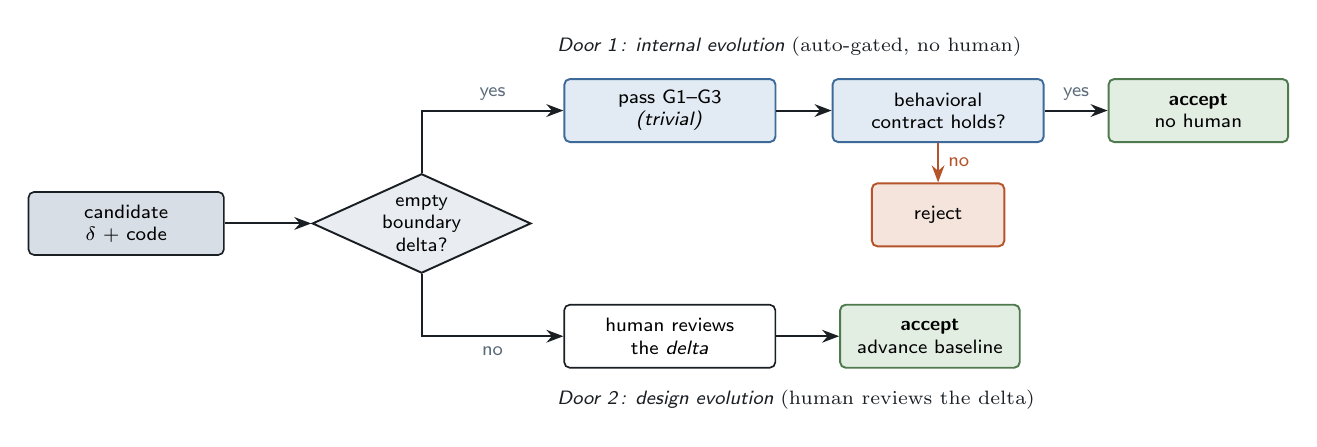
\begin{tikzpicture}[
  node distance=0pt,
  box/.style    = {rounded corners=2pt, draw=ink, line width=0.6pt, fill=white,
                   align=center, font=\sffamily\scriptsize, inner sep=4pt,
                   minimum height=8mm, text width=22mm},
  dec/.style    = {diamond, aspect=2.2, draw=ink, line width=0.7pt, fill=mist,
                   align=center, font=\sffamily\scriptsize, inner sep=1pt},
  gate/.style   = {rounded corners=2pt, draw=steel, line width=0.7pt, fill=steelwash,
                   align=center, font=\sffamily\scriptsize, inner sep=4pt,
                   minimum height=8mm, text width=24mm},
  term/.style   = {rounded corners=2pt, line width=0.7pt, align=center,
                   font=\sffamily\scriptsize, inner sep=4pt, minimum height=8mm, text width=20mm},
  flow/.style   = {->, draw=ink, line width=0.7pt},
  lbl/.style    = {font=\sffamily\scriptsize, text=slate},
  lblm/.style   = {font=\sffamily\scriptsize\itshape, text=ink},
  scale=1, transform shape,
]

%% start
\node[box, fill=mist2] (cand) at (0,0) {candidate\\ $\delta$ + code};

%% decision
\node[dec, right=11mm of cand] (dec) {empty\\ boundary\\ delta?};

%% ---- Door 1 (top): internal evolution, auto-gated ----
\node[gate, above right=7mm and 11mm of dec] (g1) {pass G1--G3\\ \emph{(trivial)}};
\node[gate, right=7mm of g1] (bc)  {behavioral\\ contract holds?};
\node[term, fill=mosswash, draw=moss, right=8mm of bc] (auto)
   {\textbf{accept}\\ no human};
\node[lblm, anchor=west] at (g1.north west |- g1.north) [yshift=4mm, xshift=-2mm] {Door 1\,: internal evolution \rmfamily\upshape(auto-gated, no human)};

%% ---- Door 2 (bottom): design evolution, human review ----
\node[box, below right=7mm and 11mm of dec, text width=24mm] (review)
   {human reviews\\ the \emph{delta}};
\node[term, fill=mosswash, draw=moss, right=8mm of review] (advance)
   {\textbf{accept}\\ advance baseline};
\node[lblm, anchor=west] at (review.south west) [yshift=-4mm, xshift=-2mm] {Door 2\,: design evolution \rmfamily\upshape(human reviews the delta)};

%% edges
\draw[flow] (cand) -- (dec);
\draw[flow] (dec.north) |- (g1.west) node[lbl, pos=0.75, above] {yes};
\draw[flow] (dec.south) |- (review.west) node[lbl, pos=0.75, below] {no};
\draw[flow] (g1) -- (bc);
\draw[flow] (bc) -- node[lbl, above] {yes} (auto);
\draw[flow] (review) -- (advance);

%% reject paths (subtle, downward)
\node[term, fill=rustwash, draw=rust, below=5mm of bc, text width=14mm] (rej1) {reject};
\draw[flow, draw=rust] (bc.south) -- node[lbl, right, text=rust] {no} (rej1.north);

\end{tikzpicture}

\caption{The two doors of evolution, selected by one predicate. A candidate
with an \emph{empty boundary delta} (Definition~\ref{def:bdelta}) is eligible
for Door~1: if the structural gates pass and the box's behavioral contract
holds, it may be accepted without human review. A candidate that touches any
boundary takes Door~2: its delta is reviewed by a human and, if approved,
advances the baseline. No proposer can reach the Door-1 fast path while
changing a boundary (Property~\ref{prop:doors}).}
\label{fig:doors}
\end{figure*}

\begin{definition}[Boundary delta]\label{def:bdelta}
The \emph{boundary delta} of a box $v$ under $G \to G'$ is the restriction of
$\Delta(G,G')$ to $v$'s public surface and the arrows incident on $v$ (in or
out). It is \emph{empty} when $\mathsf{surf}(v)$, $\mathsf{Allow}(v)$, and the
witness sets of all arrows incident on $v$ are unchanged up to $\iota$.
\end{definition}

\paragraph{Door 1: internal evolution (auto-gated).}
A change whose boundary delta is empty for every box it touches changes only
box interiors, relative to the extracted model. It is eligible for automatic
admission if it (i)~is conformant (Definition~\ref{def:conformant}) and
(ii)~preserves the behavioral contracts of the boxes it touches (concern~4).
This is the intended fast path for autonomous agents: an agent assigned the
interior of box $v$ may propose an implementation rewrite, and the gates check
that the proposal did not change the modeled boundary and did preserve the
surface obligations. \S\ref{sec:guarantees} states the assumptions under which
that is enough to justify accepting the change without human review.

\paragraph{Door 2: design evolution.}
A change with a nonempty boundary delta---a new box, a new arrow, a widened
surface, a new interface---alters the intended architecture. It produces a
graph delta that is \emph{itself} the reviewable artifact: a human (or a
higher-privilege policy) approves the \emph{delta}, which then advances the
baseline $G_\star$. Only after the boundary exists may Door-1 evolution fill in
the new box's interior.

\begin{property}[Door separation]\label{prop:doors}
The two doors use the same artifact and the same gates; they differ only in
whether the boundary delta is empty. An empty boundary delta is necessary and
sufficient for the Door-1 fast path. Consequently no proposer can perform design
evolution while claiming internal evolution: a boundary-changing proposal
\emph{cannot} take the fast path, because the emptiness check fails.
\end{property}

\noindent
Property~\ref{prop:doors} is the operational core of the safety model. It
addresses a common failure mode of automation: an optimizer reports that it only
``tuned a function'' while adding a new dependency or widening an interface. In
our regime that proposal has a nonempty boundary delta and is routed through
Door~2, where the architectural change is visible.

%% ===========================================================================
\section{Guarantees}\label{sec:guarantees}
%% ===========================================================================

We now make precise the conditional claim behind Door-1 evolution. The claim is
\emph{boundary locality}: a change confined to a box's interior, preserving its
contract, is unobservable to the rest of the system if interaction is mediated
through the box surface and the contract captures the observations contexts rely
on. We state the observational model, the assumptions, the theorem, and a proof
sketch.

\subsection{Observational model}

We treat each box $v$ as denoting a behavior $\llbracket v \rrbracket$: the
mapping from the inputs presented at its public surface to the outputs and
externally visible effects produced there. A \emph{context} $C[\cdot]$ for $v$
is the rest of the repository with a hole where $v$ sits; $C$ interacts with
$v$ \emph{only} through $\mathsf{surf}(v)$ and the arrows incident on $v$
(this is exactly what encapsulation, Definition~\ref{def:surface}, buys us).
Two boxes are \emph{observationally equivalent}, $v \approx v'$, if no
well-formed context can distinguish them:
$\forall C.\; \llbracket C[v] \rrbracket = \llbracket C[v'] \rrbracket$.

\begin{assumption}[Surface-mediated interaction]\label{asm:surface}
All interaction between a box and its context flows through the box's public
surface. Equivalently, the extractor's encapsulation (Definition~\ref{def:surface})
is sound: there is no hidden channel---no global mutable state, reflection, or
out-of-band file/network coupling---by which the context observes a box except
through $\mathsf{surf}(v)$.
\end{assumption}

\begin{assumption}[Adequate contract]\label{asm:adequate}
The behavioral contract $\mathsf{BC}(v)$ captures every surface behavior any
context relies upon: if $\mathsf{BC}(v)$ holds of two implementations, they are
interchangeable with respect to what surface observations contexts can make.
\end{assumption}

\noindent
We are deliberately explicit that these are assumptions, because they delimit
exactly where the guarantee can fail in practice---hidden channels
(Assumption~\ref{asm:surface}) and under-specified contracts
(Assumption~\ref{asm:adequate})---and \S\ref{sec:eval} and \S\ref{sec:agenda}
treat each as a measurable risk rather than a hope. Assumption~\ref{asm:surface}
is what the extractor must establish; Assumption~\ref{asm:adequate} is what
contract authoring (and its coverage) must establish.

\subsection{Boundary locality}

\begin{theorem}[Boundary locality]\label{thm:locality}
Let a change transform box $v$ into $v'$ with an \emph{empty boundary delta}
(Definition~\ref{def:bdelta}) and suppose $v'$ satisfies $\mathsf{BC}(v)$. Then
under Assumptions~\ref{asm:surface}--\ref{asm:adequate}, $v \approx v'$: for
every well-formed context $C$, $\llbracket C[v] \rrbracket = \llbracket C[v']
\rrbracket$. In particular, no other box's behavior, and no aggregated arrow or
contract elsewhere in the graph, changes.
\end{theorem}

\begin{proof}[Proof sketch]
By Definition~\ref{def:bdelta}, an empty boundary delta gives
$\mathsf{surf}(v') = \mathsf{surf}(v)$, $\mathsf{Allow}(v')=\mathsf{Allow}(v)$,
and unchanged witness sets for all arrows incident on $v$. The interface the
context binds against is therefore identical. By Assumption~\ref{asm:surface}, any
context $C$ interacts with the hole solely through that interface, so $C$'s
observations of $v$ versus $v'$ are determined entirely by the surface
behaviors $\llbracket v\rrbracket,\llbracket v'\rrbracket$ restricted to
$\mathsf{surf}(v)$. Since $v$ satisfied $\mathsf{BC}(v)$ (it is the incumbent)
and $v'$ satisfies $\mathsf{BC}(v)$ by hypothesis, Assumption~\ref{asm:adequate}
gives that the two are indistinguishable under all surface observations a
context can make. Hence $\llbracket C[v]\rrbracket = \llbracket C[v']\rrbracket$
for all $C$, i.e.\ $v\approx v'$. Because aggregated arrows
(Definition~\ref{def:agg}) and arrow contracts are functions only of leaf edges
and surface behavior at the boundary---both unchanged---nothing elsewhere in
$G$ is affected.
\end{proof}

\begin{corollary}[Compositional autonomy]\label{cor:autonomy}
Door-1 changes to \emph{disjoint} boxes compose: if agents independently rewrite
the interiors of boxes $v_1,\dots,v_k$ with no two sharing a containment-ancestor
that is also rewritten, and each preserves its contract with an empty boundary
delta, then the combined change is observationally equivalent to applying them
in any order, and to the original.
\end{corollary}

\begin{proof}[Proof sketch]
Each rewrite is unobservable to its context by Theorem~\ref{thm:locality}; in
particular each is unobservable to the other rewritten boxes, which lie in the
context. Observational equivalence is a congruence under the well-formed
contexts here (encapsulation makes box composition a context-forming operation),
so independent equivalences compose and commute.
\end{proof}

\noindent
Theorem~\ref{thm:locality} is the formal basis for the protocol in
\S\ref{sec:evolve}: the structural check establishes that the modeled boundary
did not change, and the behavioral check establishes the obligations needed to
treat the new implementation as substitutable at that boundary.
Corollary~\ref{cor:autonomy} explains when such changes can be composed across
disjoint boxes. The structural check alone is not sufficient for behavioral
safety: it shows that the \emph{interface} did not move, not that
\emph{behavior} was preserved. Where a box has \emph{no} behavioral contract,
Door~1 still provides structural locality, but the behavioral claim degrades to
the ordinary evidence supplied by the box's tests. This is not a defect in the
theorem; it is the empirical frontier the evaluation must measure.

%% ===========================================================================
\section{Evaluation Plan}\label{sec:eval}
%% ===========================================================================

The claims above require empirical support at four levels. First, the substrate
must be implementable for languages with different module and visibility
mechanisms. Second, graph deltas must be useful in real review histories, rather
than merely well defined. Third, the algebra of graphs, deltas, projections, and
gates must be tested as software, not only specified on paper. Fourth, the Door-1
protocol must be tested against agentic changes and independent behavioral
oracles. We therefore plan four linked studies: an implementation study, a
retrospective pull-request study, an executable-invariants study, and a
controlled agentic-evolution study.

\paragraph{Subjects and case studies.}
We will study large open-source repositories spanning different levels of native
boundary enforcement and different kinds of review friction. Candidate subjects
include \textsc{vLLM}, a high-velocity Python/C++/Rust inference engine with
many hardware and API surfaces; BLIS, a Go inference-simulation codebase with
explicit behavioral invariants; and Tauri, a Rust/TypeScript application
framework organized around runtime, plugin, IPC, packaging, and platform
boundaries~\cite{vllmrepo,inferencesim,taurirepo,tauriarchitecture}. For each
repository we will also select two to four implementation case-study boxes:
components with nontrivial internal logic, a stable public surface, and enough
tests or specifications to support independent behavioral checking. These boxes
are the units on which behavioral contracts and agentic rewrites will be studied.

\paragraph{Research questions.}
\begin{description}[leftmargin=2.6em,itemsep=2pt,topsep=2pt,style=sameline]
\item[\textbf{RQ1}] (Extraction) What architecture graph can be extracted with
useful precision in Python, Go, and Rust? We measure extraction coverage for
nodes, surfaces, and leaf dependencies, and manually classify missing or
spurious edges, including dynamic imports, reflection, generated code, global
state, and file or network channels.
\item[\textbf{RQ2}] (Identity) Can $\iota$ recover developer-intended renames
and moves? We measure
precision and recall of inferred correspondences against labeled refactoring
commits, and the reduction in spurious delta size compared with path-keyed
identity.
\item[\textbf{RQ3}] (Review legibility) For historical pull requests, how does
the architectural delta compare with the textual diff? We report distributions
of lines changed versus boxes, arrows, and surfaces changed at package and module
altitudes; the fraction of PRs with empty package-level deltas; and examples
where the graph delta exposes architectural risk that is hard to see in the
textual diff.
\item[\textbf{RQ4}] (Policy and migration) How would the conformance gates
classify historical changes under plausible budgets and cycle policies? We
measure pass, route-to-review, and reject classifications; identify
cycle-introducing, dependency-widening, and surface-changing PRs; and compare a
strict acyclic policy with migration policies such as strongly-connected
components as boxes, ``no new cycles,'' and ratcheting policies that require
successive graph edits to reduce architectural debt.
\item[\textbf{RQ5}] (Agentic internal evolution) On case-study boxes equipped
with behavioral contracts, do Door-1 agent rewrites that pass the structural and
behavioral gates preserve behavior under independent oracles? We measure escaped
regressions, classify each by hidden channel versus inadequate contract, and
compare against a baseline in which the agent is constrained only by the test
suite.
\item[\textbf{RQ6}] (Cost and workflow fit) What is the latency of extraction,
diffing, identity inference, and gating per push, and can the results be
presented in a form that reviewers can act on in ordinary code review and issue
triage?
\item[\textbf{RQ7}] (Executable invariants) Which ARCHON claims can be made
executable? We test graph algebra, delta computation, identity, repair edits,
and gates with generated graphs and generated changes, and we study a brownfield
system whose own behavioral invariants are being moved toward property-based
tests. We measure faults found, minimized counterexample size, and which claims
require runtime instrumentation, static checks, or type-level boundaries rather
than ordinary generated tests.
\end{description}

\paragraph{Retrospective pull-request study.}
For each subject repository, we will replay a stratified sample of historical
pull requests. The strata should include routine fixes, refactorings, dependency
changes, performance changes, and architectural reorganizations. For every PR,
we extract $G$ and $G'$, infer identity, compute graph deltas at several
altitudes, and apply the conformance gates under a small set of documented
policies. A human labeling pass will classify whether each PR is routine,
boundary-changing, or architecture-significant; this label is used to estimate
false positives and false negatives for the gate policies, not to train them.

\paragraph{Review-friction scoping study.}
Before the retrospective replay, we will sample public issues, pull requests,
and discussions in each subject repository and classify the friction they expose.
The categories should include boundary-changing refactors, cross-platform
runtime behavior, performance claims, dependency and toolchain policy, user
configuration failures, observability gaps, and low-quality agent-generated
submissions. This study is not evidence that ARCHON solves those problems. Its
purpose is to decide which frictions are architectural enough for a graph delta
to help. In BLIS, recent activity around lazy request generation and
property-tested invariants is largely architectural: the review burden is to
preserve determinism, run/replay parity, trace export, and simulator invariants
while changing the request-source boundary~\cite{blislazyrequests,blisrequestsource}.
In \textsc{vLLM}, many issues are hardware, model, or environment support, but
several high-friction changes alter stable surfaces such as sampling parameters,
multimodal render/generate payloads, and KV-transfer paths~\cite{vllmtracereplay,vllmmultimodalrfc}.
In Tauri, the recurring boundary is different again: Rust crates, JavaScript
APIs, plugin permissions, webview lifetimes, platform runtimes, bundling, and
toolchain policy~\cite{taurieventlisteners,taurimsrv}. The output of this study
is a refinement list for the extractor and contract model, especially for
non-import dependencies such as configuration keys, protocol fields, platform
labels, environment variables, and external runtime obligations.

\paragraph{Brownfield repair study.}
For repositories with visible architectural debt, we will construct a small
sequence of graph repair plans with project maintainers or expert reviewers. A
plan consists of intended graph edits, such as collapsing an SCC, extracting an
interface, forbidding a dependency, or narrowing a public surface, together with
a measurable debt objective. We then replay historical PRs, or implement focused
repair PRs, to ask whether the graph deltas make progress and regression
visible. The key measures are debt reduction per PR, number of code edits needed
per graph edit, reviewer effort to approve the graph edit, and whether the
ratchet blocks changes maintainers would consider routine.

\paragraph{Executable-invariants study.}
ARCHON's core substrate can be exercised with generated structures. We will
write property-based tests over hierarchical graphs, projected views, identity
correspondences, deltas, and repair edits. The tests should check, for
example, that projection agrees with leaf-edge witnesses, pure renames and moves
do not create spurious arrows, Door-1 eligibility fails on any boundary-changing
delta, SCC collapse preserves external arrows, and ratcheting policies do not
increase the chosen debt metric. We will also separate graph-substrate laws from
system-specific behavioral laws. Some claims, such as request conservation in a
simulator, can be tested over generated executions; others, such as ``the
proposer cannot bypass the gate'' or ``a contract cannot mention private
entities,'' are structural code-path claims. We will treat those as separate
checks, using API boundaries, access guards, or static analysis rather than
forcing them into a property-testing harness. Appendix~\ref{app:blis} sketches
BLIS as a first brownfield exemplar for this study.

\paragraph{Agentic evolution study.}
RQ5 is the load-bearing study for the conditional safety claim. For each
case-study box, we will author a behavioral contract over the public surface and
then ask one or more coding agents, and optionally a search-based proposer, to
improve an internal objective such as throughput, memory use, or code
simplification. A candidate is eligible for Door~1 only if its boundary delta is
empty and its behavioral contract holds. We then run an independent,
contract-blind oracle: property and metamorphic tests over the surface,
differential tests against the incumbent implementation, and, where feasible,
the downstream test closure of clients that use the box. Escaped regressions are
the main negative result. Each is classified as evidence of a hidden channel
(Assumption~\ref{asm:surface}) or an inadequate contract
(Assumption~\ref{asm:adequate}).

\paragraph{Implementation case studies.}
The implementation study should report where the model needed adaptation rather
than only where it succeeded. For Python, the likely issues are dynamic imports,
reflection, convention-based public surfaces, and monkey patching. For Go, the
questions are how well packages and \texttt{internal} directories approximate
the intended boxes and whether generated code introduces noisy edges. For Rust,
the questions are how crate-level visibility, features, macros, and trait
implementations affect node identity and surface extraction. These case studies
make clear which parts of \textsc{Archon} are language-neutral and which parts
are extractor engineering.

\paragraph{Metrics summary.}
Extraction precision and recall for nodes, surfaces, and edges (RQ1); identity
precision and recall and spurious-delta reduction (RQ2); delta-compression ratio,
empty-delta fraction, and reviewer-label agreement (RQ3); gate classification
rates, false positives, false negatives, and migration-policy outcomes (RQ4);
escaped regressions per accepted Door-1 change and their cause classification
(RQ5); wall-clock latency and review artifact size per PR (RQ6); property-test
coverage, minimized counterexample size, and structural-check gaps (RQ7).

%% ===========================================================================
\section{Related Work}\label{sec:related}
%% ===========================================================================

\paragraph{Modularity and dependency structure.}
The principle that modules should hide decisions likely to
change~\cite{parnas1972criteria} and that a system's value lies in the
\emph{options} its modular structure creates~\cite{baldwin2000design} is the
intellectual root of our boundary-locality claim: a stable surface is precisely
an option to change the interior freely. Design Structure
Matrices~\cite{sangal2005using} and empirical studies of dependency
structure~\cite{maccormack2006exploring} represent dependencies as a matrix
rather than a drawing and reveal cycles and modularity violations at scale; our
hierarchical graph is the same dependency relation, but versioned, per-change
diffable, and equipped with contracts, and our projection operator is the
analogue of viewing a DSM at a chosen aggregation.

\paragraph{Architecture conformance.}
Reflexion models check an implementation's dependencies against a high-level
model the architect supplies~\cite{murphy2001software}; dependency-constraint
languages and static conformance checkers~\cite{terra2009dependency,
passos2010static} enforce ``layer A may not depend on layer B'' rules in CI,
the lineage of our gate G2/G3. We differ in three ways that matter for the FSE
agenda: (i)~our intended model is \emph{derived-then-frozen} rather than
hand-authored, removing the adoption cost that has limited conformance tools in
practice; (ii)~conformance is computed on a \emph{per-change delta} at a chosen
altitude, making it a review instrument rather than a periodic audit; and
(iii)~we pair structural conformance with a \emph{behavioral} contract and a
locality \emph{theorem}, so the regime can support conditional automation rather
than only architectural hygiene.

\paragraph{Contracts and verification.}
Design by contract~\cite{beck2003contract}, property-based
testing~\cite{claessen2000quickcheck}, consumer-driven
contracts~\cite{fowler2006cdc}, and automatic verifiers~\cite{leino2010dafny}
are the techniques we attach at box surfaces (concern~4). Our contribution is
not a new verification technique but a \emph{placement discipline}: contracts
live at the public surface and nowhere else (Definition~\ref{def:bc}), because
that is the boundary at which other boxes observe the implementation.

\paragraph{Build and differencing.}
Fine-grained build systems~\cite{bazel} make per-target incrementality visible
to tooling; our per-box gating is the conformance analogue of per-target
builds. Tree-based source differencing~\cite{falleri2014finegrained} supplies
the structural-similarity signal behind our identity inference
(\S\ref{sec:identity}).

\paragraph{Automated program evolution.}
Code-generating models~\cite{chen2021codex}, agentic SWE
systems~\cite{yang2024sweagent,jimenez2024swebench}, and evolutionary
program search~\cite{romera2024funsearch,lehman2023evolution} are the
\emph{proposers} of concern~5. This literature focuses on \emph{generating}
changes; it often relies on the surrounding test suite as the main safety net.
We are complementary: \textsc{Archon} supplies an architectural boundary for
such proposers and a checkable condition, empty boundary delta plus preserved
surface contract, for deciding when a generated change should be treated as
internal rather than design-changing.

%% ===========================================================================
\section{Research Agenda and Open Questions}\label{sec:agenda}
%% ===========================================================================

This work opens questions we believe are productive for the community.

\paragraph{Contract coverage as the frontier of safe automation.}
Theorem~\ref{thm:locality} is only as strong as
Assumption~\ref{asm:adequate}. The central open question is empirical: \emph{how
much} behavioral contract must a box carry before autonomous evolution of its
interior is trustworthy, and can that coverage be grown
\emph{incrementally}---a box earning a richer contract exactly when an agent is
pointed at it? We conjecture a favorable economics: contracts are authored once
per box but amortized over unbounded agent iterations, so the cost is paid where
automation is most valuable.

\paragraph{Detecting hidden channels.}
Assumption~\ref{asm:surface} fails in the presence of global state, reflection,
or out-of-band coupling. Can extraction \emph{soundly over-approximate} these
channels---surfacing them as additional arrows so the structural gate accounts
for them---and what is the precision cost? This connects architecture
extraction to escape and effect analysis.

\paragraph{Architecture repair without a flag day.}
Many repositories do not begin with clean boundaries. They contain cycles,
informal layering violations, and APIs that exist because they were convenient
for one historical caller. The brownfield question is whether graph edits can
support a practical repair loop: identify a debt pattern in the actual graph,
declare a cleaner target graph, and admit only deltas that preserve or reduce
the distance to that target. This raises technical questions about debt metrics,
minimal repair suggestions, and how to present graph edits so maintainers review
them as design changes rather than as opaque tool output.

\paragraph{Executable architectural invariants.}
Once architecture is represented as a graph artifact, many claims become
executable. Projection, aggregation, identity, delta computation, and repair
ratchets all have algebraic properties that can be checked over generated
graphs. Other claims are structural. For example, no proposer should bypass the
gates, and a Door-1 contract should mention only the public surface of its box.
These resemble code-path invariants more than output invariants, so they require
API design, access guards, or static checks. The research question is how much
of the architecture-as-contract discipline can be made executable, and which
claims remain matters of review and evidence.

\paragraph{Operational contracts beyond imports.}
The case-study repositories show that many review-relevant boundaries are not
ordinary source dependencies. \textsc{vLLM} changes often hinge on API fields,
runtime flags, backend dispatch, hardware paths, and numerical tolerances. Tauri
changes often hinge on platform labels, webview lifetimes, plugin permissions,
bundling metadata, and upstream runtime behavior. BLIS changes often hinge on
observability fields and replay determinism. ARCHON therefore needs a typed
edge model: import edges are only one class of arrow. Configuration, protocol,
capability, platform, metric, and observability edges should be represented as
first-class architectural facts when they are the boundary reviewers care about.

\paragraph{The aggregation of contracts.}
We chose to restate a parent's behavioral contract independently rather than
derive it from its children (\S\ref{sec:contracts}). When is a sound
\emph{compositional} contract derivable, so that verifying children suffices to
verify the parent? This is the hierarchical-verification question, and a
positive answer would let safe automation climb the containment tree.

\paragraph{Fitness and the evolution loop.}
We deliberately fixed the substrate and left the proposer open. A full study of
\emph{which} evolutionary loops (LLM agents, search, hybrid) best exploit the
boundary---and how the fitness signal interacts with the safety gates---is
future work that the substrate is designed to enable rather than prejudge.

\paragraph{Threats to validity.}
The boundary-locality result is conditioned on
Assumptions~\ref{asm:surface}--\ref{asm:adequate}; where they fail, Door~1
degrades to the evidence supplied by ordinary tests. Identity inference bounds
legibility but, as noted, not the soundness of the post-change gates.
Generalization beyond the three studied languages, and to repositories whose
architecture is genuinely a non-hierarchical web, are open empirical risks; the
projection operator assumes a containment tree exists, which holds for the
package systems of Go, Rust, and Python but may not for all artifacts.

%% ===========================================================================
\section{Conclusion}\label{sec:conclusion}
%% ===========================================================================

Engineers have long drawn their systems as boxes and arrows. We argued that, in
large repositories increasingly changed by both humans and machines, that view
should become a checked, versioned artifact: one object serving as documentation,
review lens, and contract boundary for automated proposers. We gave a
hierarchical attributed graph that reconciles human package-level review and
agent function-level edits as projections of one structure, a notion of node
identity stable under refactoring, and a conformance regime built around graph
deltas. The technical core is a conditional boundary-locality result: if the
modeled boundary does not change and the surface contract is preserved, then
under explicit assumptions the implementation change is unobservable outside the
box. The next step is empirical. Building \textsc{Archon} and studying it on
real monorepos will show which parts of the model are practical today, where
extractors lose precision, and how much behavioral contract coverage is needed
before autonomous internal evolution is a defensible engineering practice.

\appendix

%% ===========================================================================
\section{Candidate Brownfield Exemplars}\label{app:exemplars}
%% ===========================================================================

This appendix records three initial brownfield exemplars for the empirical
study. They are not meant to be exhaustive. BLIS stresses executable invariants
and ratcheting, \textsc{vLLM} stresses high-velocity review around serving
surfaces, and Tauri stresses platform, plugin, lifecycle, and toolchain
boundaries. Additional greenfield exemplars should be added later to test the
contract-first path.

\subsection{BLIS: executable invariants and ratcheting}
\label{app:blis}

BLIS is useful because it was not constructed for this paper. The public
artifacts include the Go \texttt{inference-sim} simulator and a related Python
calibration artifact for trace-only step-level coefficient
estimation~\cite{inferencesim,blisrepo}. The
simulator documentation names system invariants such as request conservation,
clock monotonicity, KV-cache conservation, lifecycle causality, determinism,
signal freshness, work conservation, oracle-knowledge boundaries, session
completeness, and preemption completeness~\cite{blisinvariants}. A public design
discussion proposes turning those invariants into property-based tests using
\texttt{rapid}, together with Go fuzz targets for parsers, KV allocation, batch
formation, and admission~\cite{blispropertydiscussion}.

This makes BLIS a brownfield case in the sense relevant to ARCHON. The
invariants were written after substantial system behavior already existed, and
some proposed checks cannot yet be automated because the simulator lacks the
observability fields needed to expose the relevant facts~\cite{blisobservability}.
That is exactly the adoption problem a graph substrate should handle: capture
the current design, expose the missing boundary and instrumentation facts, and
ratchet toward a cleaner target. BLIS also separates three kinds of claims that
ARCHON must keep distinct. Some are conservation identities, such as request or
KV-cache conservation. Some are ordering properties, such as clock monotonicity
and lifecycle causality. Others are structural code-path properties, such as the
rule that admission must not read oracle output tokens. The first two fit
property-based testing over generated simulation configurations. The third needs
API boundaries, access guards, or static checks.

An ARCHON study would use BLIS in two complementary ways. At the architecture
level, we would extract boxes for routing, scheduling, KV state, workload
generation, session management, metrics, and trace replay, then replay
historical changes to ask whether architectural deltas expose the same boundary
issues the invariant documents name. At the executable-invariant level, we would
translate selected ARCHON graph laws into generated tests: projection agrees
with leaf-edge witnesses, repair edits preserve external arrows, Door-1 routing
fails on boundary deltas, and behavioral contracts mention only public-surface
entities. The BLIS invariants provide the exemplar's behavioral side: generated
simulation configurations check conservation, causality, and determinism, while
structural guards enforce oracle-knowledge boundaries.

The point is not that BLIS alone validates ARCHON. It is a first brownfield case
in a broader exemplar set. A later greenfield exemplar should start with an
intended graph and executable invariants before implementation, so we can compare
the two adoption paths: snapshot-and-ratchet for brownfield systems, and
contract-first construction for greenfield systems.

\subsection{\textsc{vLLM}: review at high velocity}
\label{app:vllm}

\textsc{vLLM} stresses a different part of ARCHON. The project receives a large
volume of issue and pull-request activity across Python, C++, Rust, CUDA, ROCm,
CPU, XPU, frontend APIs, multimodal serving, KV transfer, and CI/build
infrastructure~\cite{vllmrepo}. Much of this friction is not architectural in
ARCHON's sense: a driver mismatch, a model-specific template bug, or an
environment-specific build failure still needs domain debugging. The relevant
question is narrower: when does a change alter a surface that many contributors
and users rely on, and can that fact be made visible before reviewers infer it
from a large textual diff?

Two recent examples illustrate the fit. A trace-replay proposal adds a
\texttt{trace\_decode\_token\_ids} field to sampling parameters and threads that
obligation through sampler injection, request admission, and engine-core state
so a fixed decode trace can be replayed while preserving real logprob
computation~\cite{vllmtracereplay}. This is a boundary change: the public
sampling surface grows, and the internal implementation must preserve a
behavioral contract about forced tokens and unmodified logits. A multimodal RFC
argues that the token-in/token-out path should avoid sending large preprocessed
\texttt{pixel\_values} payloads from \texttt{/render} to
\texttt{/generate}; the real design question is where preprocessing belongs and
which cache/routing metadata must remain stable~\cite{vllmmultimodalrfc}. Both
cases suggest that ARCHON must model protocol fields, API parameters, route
semantics, and backend dispatch edges, not only import edges.

\subsection{Tauri: platform and plugin boundaries}
\label{app:tauri}

Tauri is a Rust/TypeScript framework whose own architecture document separates
core crates, build-time code generation, runtime abstractions, WRY-specific
runtime integration, JavaScript APIs, CLI tooling, bundling, plugins, and
upstream TAO/WRY dependencies~\cite{taurirepo,tauriarchitecture}. Its public
activity shows a third kind of friction. Many issues are platform-specific:
Windows WebView2 behavior, Android path resolution, macOS signing or ACL
snapshots, Linux tray and Wayland behavior, and WSL/development-environment
setup. Others concern framework boundaries: command registration, plugin
ownership, event listeners tied to webview lifetimes, capability permissions,
updater metadata, and MSRV policy~\cite{taurieventlisteners,taurimsrv}.

ARCHON would not make platform-specific behavior disappear. It can, however,
make the review surface explicit. A stale-listener issue is not just a memory
bug; it names a lifecycle contract between JavaScript listeners, webview
destruction, and backend listener maps~\cite{taurieventlisteners}. An MSRV RFC
is not a code dependency edge; it is a toolchain-policy contract that constrains
all crates and dependency updates~\cite{taurimsrv}. Tauri therefore pushes
ARCHON toward typed operational edges: plugin-command edges, capability edges,
platform-support edges, toolchain-policy edges, and upstream-runtime edges. It
also provides a useful stress test for agentic evolution, because some recent
activity is explicitly labeled as low-quality AI-generated contribution; an
ARCHON gate could route such changes by boundary impact and missing evidence
rather than by authorship alone~\cite{tauriaislop}.

\bibliographystyle{ACM-Reference-Format}
\bibliography{refs}

\end{document}
